% -*- TeX:EN -*-
\PassOptionsToPackage{hyphens}{url}
\input{FX_plain_en_20201026}

%% 0) declaration:
\newread\verfilein \newwrite\verfileout  \newcount\vernum

%% 1) reading the file:
\openin\verfilein="eduino.ver"
\ifeof\verfilein \def\tmp{0}\else \read\verfilein to\tmp \fi
\closein\verfilein
\vernum=\tmp

%% 2) adding +1
\advance\vernum by1
\edef\thevernum{\the\vernum}

%% 3) saving the value to the file:
\immediate\openout\verfileout="eduino.ver"
\immediate\write\verfileout{\the\vernum}
\immediate\closeout\verfileout

\counterwithout{figure}{chapter}
   \counterwithout{table}{chapter}

   \captionnamefont{\small\slshape\color{RoyalBlue4}}
   \captiontitlefont{\small\slshape\color{RoyalBlue4}}
\newfontfamily\titlefont{Lucida Sans}

\begin{document}\sisetup{math-micro=\text{µ},text-micro=µ,output-decimal-marker={.}}
\setcounter{page}{1}\thispagestyle{empty}

\makeatletter
\renewcommand\tableofcontents{%
\begin{multicols}{2}%[
    \@starttoc{toc}%
\end{multicols}}
\makeatother


\mainmatter
%  \renewcommand{\bibsection}{\section*{\refname}}
  \renewcommand{\bibsection}{}
  \counterwithout{figure}{chapter}
  \counterwithout{table}{chapter}
  \counterwithout{footnote}{chapter}

\noindent{\titlefont\Huge Eduino\\[1ex] A better ATmega32U4 breakout board\\}

%  \begin{tikzpicture}[remember picture,overlay]
%    \fill[yellow] ($(current page.north east)-(30mm,0mm)$) -- ($(current page.north east)-(60mm,0mm)$) -- ($(current page.north east)-(0mm,60mm)$) -- ($(current page.north east)-(0mm,30mm)$) -- ($(current page.north east)-(30mm,0mm)$);
%    \path ($(current page.north east)-(45mm,0mm)$) -- ($(current page.north east)-(0mm,45mm)$) node[pos=0.5,anchor=center,rotate=-45,text width=5cm,align=center]{\Large\bfseries New 2020\\[.5ex] beta release};
%  \end{tikzpicture}

\noindent\rule{17cm}{0.5mm}
\begin{flushright}
 doc version \thevernum,  \today
\end{flushright}

\sisetup{retain-unity-mantissa = false,retain-zero-exponent = true}
The goal of this project was to come up with a replacement for the campus lab exercises in the courses
1TE663 and 1TE723 on
microcontroller programming at Uppsala University during the Corona fall semester of 2020.

\section*{Contents}
\tableofcontents

\clearpage

\begin{multicols}{2}
\section{Background}
During the history of the course I have migrated from using an Atmel STK500 to using bare
ATmega328 chips on solderless breadboards together with an USB-attached serial programmer.
Originally a commercial programmer before I introduced my own design which plugged right
into the power rail of the breadboard.

However, getting everything to work for all students even in on-site labs was not easy:
\begin{itemize}\tightlist
  \item the necessary drivers would repeatedly disappear from Windows installations
  \item there was no
direct way of communicating back from the program code on the microcontroller to the host
computer without additional hardware
  \item wiring 5 cables between the programmer and the microcontroller could be done in
  120 different combinations, of which only one is correct
\end{itemize}

When I got the idea of home-labs early summer 2020 I started looking into the \emph{Pro Micro} (see Fig.~\ref{fig.promicro})
platform, originally developed by \emph{Spark Fun}, based on the \emph{Arduino} \emph{Leonardo}.
I liked the idea of utilizing a microcontroller
with built-in USB interface which can directly connect to any modern operating system
since it can emulate a CDC-type serial interface which does not need any additional drivers under
either Windows, MacOS or Linux.

However, I found the \emph{Pro Micro} itself quite unattractive for the course. The reasons
can be found in the schematic diagram of the \emph{Pro Micro} (see Fig.~\ref{fig.promicro_sch}):
\begin{itemize}\tightlist
  \item out of the 26 GPIO pins of the ATmega32U4 (see Fig.~\ref{fig.m32u4_chip}) only 18 are available
  \item no complete 8-bit port is available, since PB0 and PD5 are misused for one of the on-board LEDs, and PB7 and PD6 are ``not used''
  \item the SPI-interface is not fully functional, because pin SS or PB0 is used for the LED
  \item all pins are more or less randomly placed on the pinheaders
\end{itemize}

\begin{figure*}[p]
  \centering
  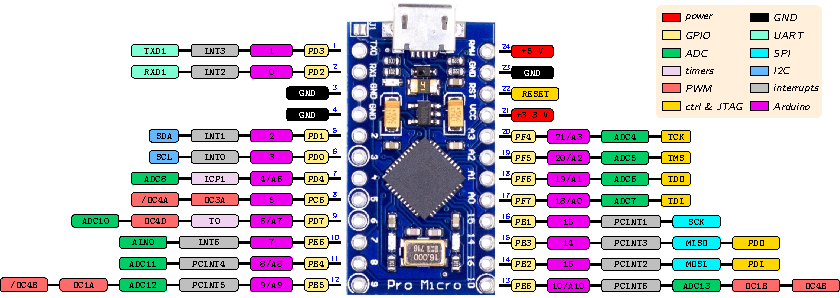
\includegraphics[width=.9\textwidth]{arduino_promicro_pinout}
  \caption{Pinout of the \emph{Pro Micro} by \emph{Spark Fun}.}\label{fig.promicro}
\end{figure*}

\begin{figure*}[p]
  \centering
  \includegraphics[clip=true,trim= 3mm 42mm 85mm 35mm,width=\textwidth]{Pro_Micro_v13b}
  \caption{Schematic diagram of the \emph{Pro Micro} by \emph{Spark Fun}.}\label{fig.promicro_sch}
\end{figure*}

\section{Design phase}
Designing the circuit board for the Eduino took about 2 days during my summer vacation.
I had the goal to
\begin{itemize}\tightlist
  \item make all 8 pins of ports \lstinline!B! and \lstinline!D! available, like on the ATmega328
  \item sort the pins according to their bit-values in the ports
  \item make as many of the other pins available as possible
  \item use \SI{3.3}{\volt} as the main supply voltage for compatibility with modern peripherals
  \item don't hide anything from view and use a clean layout with labels for all parts
\end{itemize}
The design was done in KiCAD v5 and I took the opportunity to order a few boards both assembled and
unassembled from \emph{PCBgogo} in Shenzhen in China. It was my first order of preassembled boards and
I wanted to see what they could offer and how much it would cost.

I made one mistake by not reading the datasheet of the ATmega32U4 too carefully. For \SI{3.3}{\volt} operation
the datasheet forbids the use of a \SI{16}{\mega\hertz} quartz resonator but would allow the use
of \SI{12}{\mega\hertz}. So this was my choice, but I then had to figure out that the USB
interface requires the use of either \SI{8}{\mega\hertz} or \SI{16}{\mega\hertz}. Therefore I had to
replace the surface mounted quartz resonators (part Y1) from the first units.

\section{Design challenges}
Drawing up the schematic diagram of the circuit around the ATmega32U4 was not a big
issue, see Fig.~\ref{fig.m32u4_sch}. I started with the USB interface and the power supply part. Since I wanted to
have as many pins available as possible I decided to go with a single LED on the board
apart from a power-indicator LED. Pin \lstinline!PE6! is quite lonely on port \lstinline!E! of the ATmega32U4 since
the only other pin from port \lstinline!E!, \lstinline!PE2!, is signalling the use of the bootloader code after a reset.
I would have to change the bootloader code to use a single LED on \lstinline!PE6! then instead of using the
two LEDs on \lstinline!PB0! and \lstinline!PD5!, but that can be easily done.

\begin{figure}[H]
  \centering
  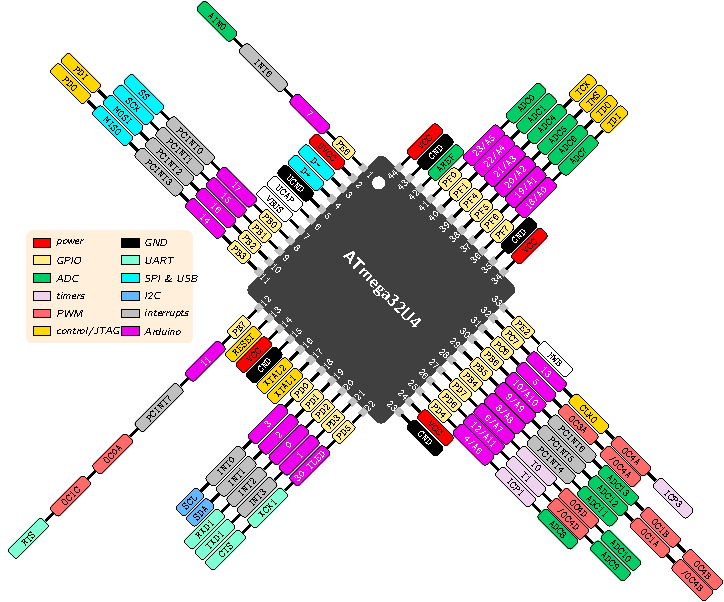
\includegraphics[width=\columnwidth]{20230210_atmega32u4_tqfp}
  \caption{Pinout of the ATmega32U4 microcontroller.}\label{fig.m32u4_chip}
\end{figure}

The \emph{Pro Micro} itself has two pin headers with 12 pins each. With 26 GPIO pins available
for my design plus the need of power supply pins it was clear that I would need more pins.
When laying out the circuit I ended up with two pin headers with 16 pins each for a total
of 32 connection points.

The real obstacle came then when looking at the pinout of the ATmega32U4 itself, see Fig.~\ref{fig.m32u4_chip}.
To my surprise
the pins on the 44-pin package of the chip were by far not as nicely sorted as
on an ATmega16, ATmega328 och ATmega644, to which I was used from the past. Just as an example,
why are the pins from port \lstinline!D! not sorted in order, but rather pins \lstinline!PD4! and \lstinline!PD5!
 are swapped? Why are
three pins from port \lstinline!B! on the wrong side of the package?

I understand that it most probably made the layout of the actual chip inside the package easier
for the designers at \emph{Microchip} (or at \emph{Atmel} at that time), but really?

Still it was possible to untangle this maze on a two-layer PCB (see Fig.~\ref{fig.m32u4_board}), but in order to make my own work
not to complicated I decided to go for the maximum width of the board at \SI{26}{\milli\metre} which would fit onto a
standard solderless breadboard, leaving one column of holes accessible on each side. The final arrangement of the pins on the
breakout board can be seen in Fig.~\ref{fig.m32u4_pinout}.

\begin{figure}[H]
  \centering
  \begin{tikzpicture}
    \path(0,0)node[anchor=south east,inner sep=1mm](front){\includegraphics[clip=true,trim= 135mm 76mm 135mm 87mm,width=.45\columnwidth]{20200622_m32u4-F_Cu}};
    \path(0,0)node[anchor=south west,inner sep=1mm](back){\includegraphics[clip=true,trim= 135mm 76mm 135mm 87mm,width=.45\columnwidth]{20200622_m32u4-B_Cu}};
    \path(front.south)node[anchor=north]{front side};
    \path(back.south)node[anchor=north]{back side};
  \end{tikzpicture}
  \caption{Copper layers of the breakout board. The USB connector is at the top and the back side is mirrored horizontally to line up with the front side.}\label{fig.m32u4_board}
\end{figure}

\begin{figure*}
  \centering
  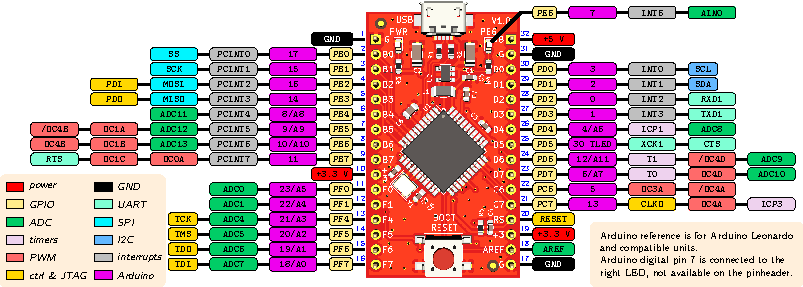
\includegraphics[width=\textwidth]{20230210_eduino_pinout}
  \caption{Pinout of the breakout board.}\label{fig.m32u4_pinout}
\end{figure*}

\begin{figure*}
  \centering
  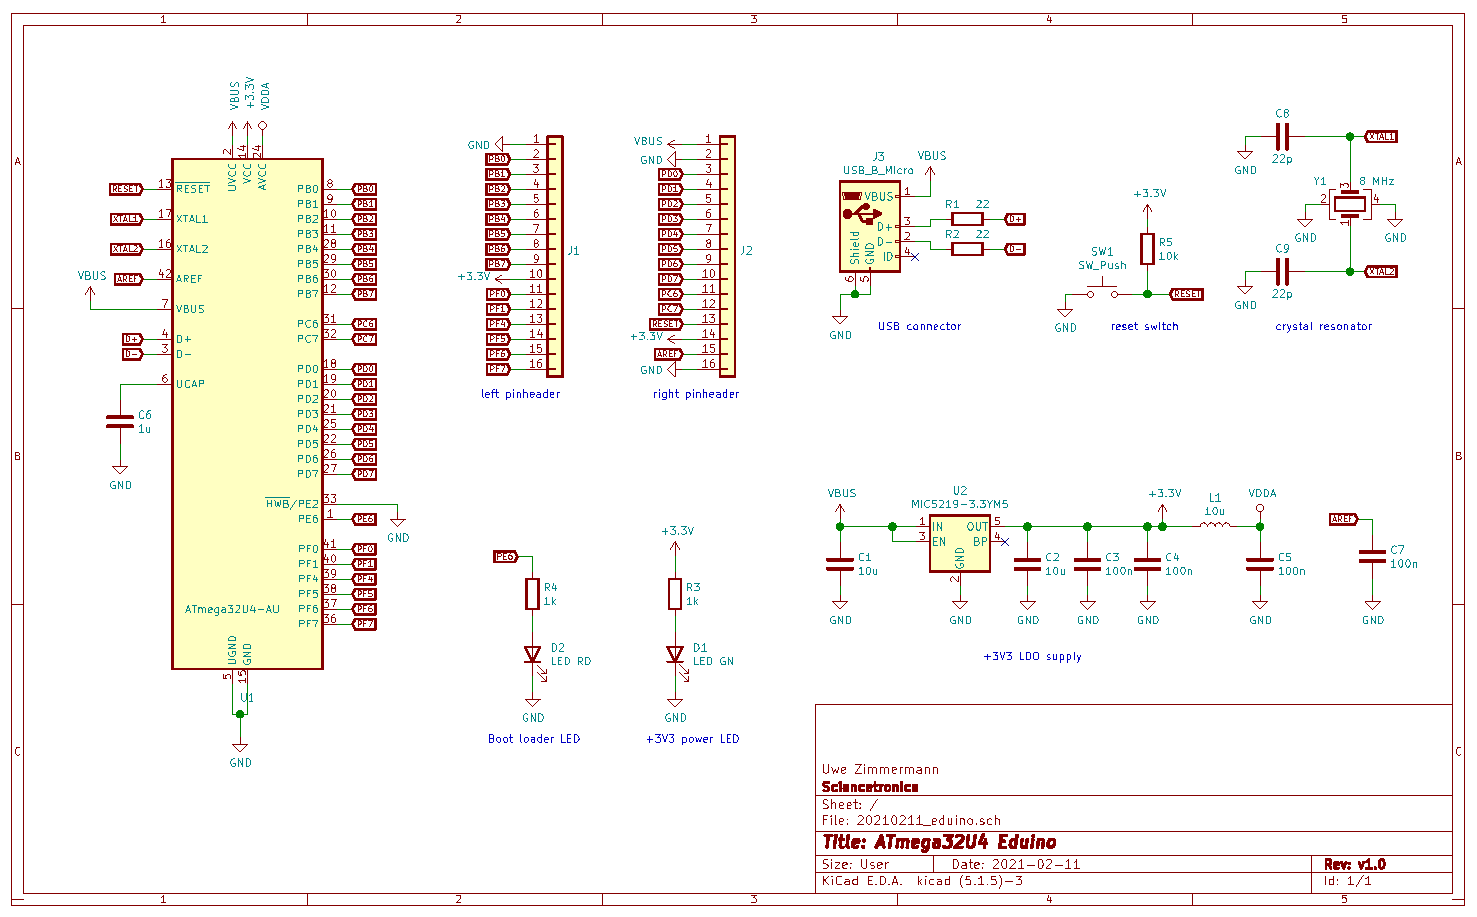
\includegraphics[width=\textwidth]{20210211_eduino}
  \caption{Schematic diagram of the breakout board.}\label{fig.m32u4_sch}
\end{figure*}

\section{Parts}
\begin{tabbing}
~~\=\hspace*{15mm}\=\hspace*{35mm}\=  \kill
Resistors \+\\
  R1 \> \SI{22}{\ohm} \> 0603 \\
  R2 \> \SI{22}{\ohm} \> 0603 \\
  R3 \> \SI{1}{\kilo\ohm} \> 0603 \\
  R4 \> \SI{1}{\kilo\ohm} \> 0603 \\
  R5 \> \SI{10}{\kilo\ohm} \> 0603 \\
  \-\\
Capacitors \+\\
  C1 \> \SI{10}{\micro\farad}, \SI{16}{\volt} \> 1206 \\
  C2 \> \SI{10}{\micro\farad}, \SI{16}{\volt} \> 1206 \\
  C3 \> \SI{100}{\nano\farad}, \SI{16}{\volt} \> 0603 \\
  C4 \> \SI{100}{\nano\farad}, \SI{16}{\volt} \> 0603 \\
  C5 \> \SI{100}{\nano\farad}, \SI{16}{\volt} \> 0603 \\
  C6 \> \SI{1}{\micro\farad}, \SI{16}{\volt} \> 0805 \\
  C7 \> \SI{100}{\nano\farad}, \SI{16}{\volt} \> 0603 \\
  C8 \> \SI{22}{\pico\farad}, \SI{16}{\volt} \> 0603 \\
  C9 \> \SI{22}{\pico\farad}, \SI{16}{\volt} \> 0603 \\
  \-\\
Inductors  \+\\
  L1 \> \SI{10}{\micro\henry} \> 1206 \\
  \-\\
LEDs  \+\\
  D1 \> LED green \> 0603 \\
  D2 \> LED red \> 0603 \\
  \-\\
Integrated circuits \+\\
  U1 \> ATmega32U4-AU \> TQFP44\\
  U2 \> MIC5219-3.3YM5 \> SOT23-5\\
  \-\\
Crystals\+\\
  Y1 \> \SI{8}{\mega\hertz} xtal \> 3225-4\\
  \-\\
Electromechanical\+\\
  SW1 \> push button \> 6x6mm 4pin\\
  J1 \> pinheader \> 16x2.56mm\\
  J2 \> pinheader \> 16x2.56mm\\
  J3 \> micro-USB \> C40942\\
\end{tabbing}


\section{Architecture}
\subsection{USB connection}
  The ATmega32U4 contains all the hardware for a full speed USB-2 interface,
  including the differential drivers, supply voltage control, timing and
  pull-up resistors.

  In order to use the hardware USB-interface, the microcontroller has to be
  clocked with \SI{8}{\mega\hertz} or \SI{16}{\mega\hertz}, an internal PLL
  (phase locked loop) generates the necessary timing for the data transfer.

\subsection{Supply voltage}
  The breakout board is supplied via the USB cable from either an attached computer,
  a power bank or a wall adapter. The USB supply voltage of nominally \SI{5}{\volt}
  is directly available on pin 32 of the breakout board, with the corresponding GND
  at pins 1, 17 and 31.

  The ATmega32U4 itself is supplied through a LDO (low dropout) regulator with
  a \SI{3.3}{\volt} supply voltage which is available on pins 10 and 19 of the
  breakout board for the connection of external sensors, peripherals, etc.

  On pin 18 of the brakout board the \lstinline!AREF! pin of the ATmega32U4 is available
  for the possible connection of an external voltage reference or to be used as a
  voltage reference of an external circuit.

\subsection{PORT B}
  Port B of the ATmega32U4 is an 8-bit GPIO port with individual control over
  all 8 pins \lstinline!PB0! to \lstinline!PB7!. Data direction is controlled via the \lstinline!DDRB!
  register, output data is sent to the \lstinline!PORTB! register and
  data from the outside is read via the \lstinline!PINB! register.

  Some pins of port B have additional functional layers:
  \begin{itemize}\tightlist
    \item \lstinline!PB0! to \lstinline!PB3! are alternatively used by the SPI interface and for serial programming of the chip
    \item \lstinline!PB4! to \lstinline!PB6! can also be used as additional analog inputs for the internal ADC
    \item \lstinline!PB5! to \lstinline!PB7! can also carry PWM signals generated by timer 0, 1 and 4
    \item \lstinline!PB7! is also used as control signal \lstinline!RTS! in full UART operation
  \end{itemize}

\subsection{PORT C}
  Port C of the ATmega32U4 is internally an 8-bit GPIO port, but only pins \lstinline!PC6! and \lstinline!PC7!
  are available on the outside of the package. Data direction is controlled via the \lstinline!DDRC!
  register, output data is sent to the \lstinline!PORTC! register and
  data from the outside is read via the \lstinline!PINC! register.

  The pins of port C have additional functional layers:
  \begin{itemize}\tightlist
    \item \lstinline!PC6! and \lstinline!PC7! can also carry PWM signals generated by timer 3 and 4
    \item \lstinline!PC7! can be used an output pin for the internal CPU clock
    \item \lstinline!PC7! can also be used as a capture signal input for timer 3
  \end{itemize}

\subsection{PORT D}
  Port D of the ATmega32U4 is an 8-bit GPIO port with individual control over
  all 8 pins \lstinline!PD0! to \lstinline!PD7!. Data direction is controlled via the \lstinline!DDRD!
  register, output data is sent to the \lstinline!PORTD! register and
  data from the outside is read via the \lstinline!PIND! register.

  Some pins of port B have additional functional layers:
  \begin{itemize}\tightlist
    \item \lstinline!PD0! and \lstinline!PD1! are alternatively used by the I2C or TWI interface
    \item \lstinline!PD2!, \lstinline!PD3! and \lstinline!PD5! are used by the UART interface
    \item \lstinline!PD4!, \lstinline!PD6! and \lstinline!PD7! can also be used as additional analog inputs for the internal ADC
    \item \lstinline!PD4! can also be used as a capture signal input for timer 1
    \item \lstinline!PD6! can be used as an external clock source for timer 1
    \item \lstinline!PD7! can be used as an external clock source for timer 0
  \end{itemize}


\subsection{PORT E}
  Port E of the ATmega32U4 is an 8-bit GPIO port, but only pins \lstinline!PE2! and \lstinline!PE6!
  are available on the outside of the package. Data direction is controlled via the \lstinline!DDRE!
  register, output data is sent to the \lstinline!PORTE! register and
  data from the outside is read via the \lstinline!PINE! register.

  The breakout board does not give access to either of these pins.
  \begin{itemize}\tightlist
    \item \lstinline!PE2! is tied to ground to enable the use of the internal bootloader
    \item \lstinline!PE6! is hardwired to the red status LED on the board
  \end{itemize}

\subsection{PORT F}
  Port F of the ATmega32U4 is internally an 8-bit GPIO port, but only pins \lstinline!PF0!, \lstinline!PF1!
  and \lstinline!PF4! to \lstinline!PF7!
  are available on the outside of the package. Data direction is controlled via the \lstinline!DDRF!
  register, output data is sent to the \lstinline!PORTF! register and
  data from the outside is read via the \lstinline!PINF! register.

  The pins of port C have additional functional layers:
  \begin{itemize}\tightlist
    \item all pins on port F can also be used as additional analog inputs for the internal ADC
    \item \lstinline!PF4! to \lstinline!PF7! are used for the JTAG interface -- if enabled
  \end{itemize}

\section{Bootloader}
  The \emph{Caterina} bootloader is activated by a double-click of the reset button
  on the breakout board. When in bootloader mode the \lstinline!PE6! LED signals a
  pumping flash and the breakout board can be recogninzed on an attached computer as
  a CDC-compatible serial port. The bootloader will timeout after about \SI{8}{\second}
  and normal program execution will restart if no connection from a host computer is made.

  Uploaders like \lstinline!avrdude! need to be provided with the address of
  this serial port (\lstinline!COMxx! under Windows, \lstinline!/dev/ttyXX! or similar under
  MacOS and Linux) in order to connect to the ATmega32U4 and be able to upload new program code
  into the flash memory.

  The breakout boards are preliminary identifying themselves with a \lstinline!VID! of \lstinline!0x1B4F!
  and a \lstinline!PID! of \lstinline!0x9205! as a \emph{Spark Fun} 5V \emph{Pro Micro} to which
  they are mostly compatible,
  apart from the lower clock frequency of \SI{8}{\mega\hertz} -- but this is not relevant for the
  functioning of the bootloader.


\section{CDC serial port}
  The USB connection can also be used for a continuous serial data connection to a host computer
  during the normal program execution. For this a separate library, the \emph{M2 USB communication subsystem} by
  J.\ Fiene \& J.\ Romano is recommended and will be used during the course.
\end{multicols}

\section*{External links}
\begin{itemize}
  \item Schematic drawing of the \emph{Pro Micro} from \emph{Spark Fun}\\ \url{https://cdn.sparkfun.com/datasheets/Dev/Arduino/Boards/Pro_Micro_v13b.pdf}
  \item ATmega32U4 datasheet\\ \url{http://ww1.microchip.com/downloads/en/DeviceDoc/Atmel-7766-8-bit-AVR-ATmega16U4-32U4_Datasheet.pdf}
  \item The original \emph{Caterina} bootloader by Dean Camera on GitHub\\
      \url{https://github.com/adafruit/Caterina-Bootloader}
  \item \emph{M2 USB communication subsystem} by J. Fiene \& J. Romano\\
  \url{http://medesign.seas.upenn.edu/index.php/Guides/MaEvArM-usb}
\end{itemize}
\end{document}

%
\begin{xtabular*}{\columnwidth}{lrl}
  R1 & \SI{22}{\ohm} & 0805 \\
  R2 & \SI{22}{\ohm} & 0805 \\
  R3 & \SI{1}{\kilo\ohm} & 0805 \\
  R4 & \SI{1}{\kilo\ohm} & 0805 \\
  R5 & \SI{10}{\kilo\ohm} & 0805 \\
  \hline
  C1 & \SI{10}{\micro\farad}, \SI{16}{\volt} & 1206 \\
  C2 & \SI{10}{\micro\farad}, \SI{16}{\volt} & 1206 \\
  C3 & \SI{100}{\nano\farad}, \SI{16}{\volt} & 0805 \\
  C4 & \SI{100}{\nano\farad}, \SI{16}{\volt} & 0805 \\
  C5 & \SI{100}{\nano\farad}, \SI{16}{\volt} & 0805 \\
  C6 & \SI{1}{\micro\farad}, \SI{16}{\volt} & 0805 \\
  C7 & \SI{100}{\nano\farad}, \SI{16}{\volt} & 0805 \\
  C8 & \SI{22}{\pico\farad}, \SI{16}{\volt} & 0805 \\
  C9 & \SI{22}{\pico\farad}, \SI{16}{\volt} & 0805 \\
  \hline
  D1 & LED green & 0805 \\
  D2 & LED red & 0805 \\
  \hline
  U1 & ATmega32U4-AU & TQFP44\\
  U2 & MIC5219-3.3YM5 & SOT23-5\\
  \hline
  Y1 & \SI{8}{\mega\hertz} xtal & 3225-4\\
  \hline
  SW1 & push button & 6x6mm 4pin\\
  J1 & pinheader & 16x2.56mm\\
  J2 & pinheader & 16x2.56mm\\
  J3 & micro-USB & C40942\\
\end{xtabular*}

